\documentclass[12pt, a4paper]{article}

% ============================================================
% Packages
% ============================================================
\usepackage[utf8]{inputenc}
\usepackage[T1]{fontenc}
\usepackage{amsmath, amssymb, amsthm}
\usepackage{mathrsfs}
\usepackage{hyperref}
\usepackage{cleveref}
\usepackage{enumitem}
\usepackage{booktabs}
\usepackage{listings}
\usepackage{xcolor}
\usepackage[margin=1in]{geometry}
\usepackage{tikz}
\usetikzlibrary{positioning, arrows.meta, calc}

% ============================================================
% Theorem Environments
% ============================================================
\theoremstyle{plain}
\newtheorem{theorem}{Theorem}[section]
\newtheorem{lemma}[theorem]{Lemma}
\newtheorem{proposition}[theorem]{Proposition}
\newtheorem{corollary}[theorem]{Corollary}

\theoremstyle{definition}
\newtheorem{definition}[theorem]{Definition}
\newtheorem{example}[theorem]{Example}

\theoremstyle{remark}
\newtheorem{remark}[theorem]{Remark}

% ============================================================
% Lean 4 Listings
% ============================================================
\lstdefinelanguage{Lean4}{
  morekeywords={theorem, def, lemma, axiom, opaque, noncomputable,
    import, open, where, instance, structure, inductive, deriving,
    if, then, else, match, with, fun, let, have, show, by,
    exact, rfl, intro, cases, constructor, unfold, rw, simp,
    contradiction, absurd, decide, refine, Prop, Type, Bool,
    true, false, Nat, sorry},
  sensitive=true,
  morecomment=[l]{--},
  morecomment=[s]{/-}{-/},
  morestring=[b]",
  literate={→}{$\to$}1 {←}{$\leftarrow$}1 {↔}{$\leftrightarrow$}1
           {∧}{$\wedge$}1 {∨}{$\vee$}1 {¬}{$\neg$}1
           {≤}{$\le$}1 {≥}{$\ge$}1 {≠}{$\ne$}1
           {⟨}{$\langle$}1 {⟩}{$\rangle$}1
           {∀}{$\forall$}1 {∃}{$\exists$}1
           {ℕ}{$\mathbb{N}$}1 {ℤ}{$\mathbb{Z}$}1
           {ℚ}{$\mathbb{Q}$}1 {ℝ}{$\mathbb{R}$}1
}

\lstset{
  language=Lean4,
  basicstyle=\ttfamily\small,
  keywordstyle=\bfseries\color{blue!60!black},
  commentstyle=\itshape\color{green!40!black},
  stringstyle=\color{red!60!black},
  breaklines=true,
  columns=flexible,
  frame=single,
  framerule=0.4pt,
  xleftmargin=1em,
  numbers=left,
  numberstyle=\tiny\color{gray},
  numbersep=5pt
}

% ============================================================
% Notation
% ============================================================
\newcommand{\BISH}{\mathrm{BISH}}
\newcommand{\BISHMP}{\mathrm{BISH{+}MP}}
\newcommand{\LLPO}{\mathrm{LLPO}}
\newcommand{\WLPO}{\mathrm{WLPO}}
\newcommand{\LPO}{\mathrm{LPO}}
\newcommand{\CLASS}{\mathrm{CLASS}}
\newcommand{\CRM}{\mathrm{CRM}}
\newcommand{\DPT}{\mathrm{DPT}}
\newcommand{\Qell}{\mathbb{Q}_\ell}

% ============================================================
\title{Standard Conjecture~D Is Necessary\\
for Constructive Morphism Decidability\\[6pt]
\large (Paper~73, Constructive Reverse Mathematics Series)}

\author{Paul Chun-Kit Lee\\
\small New York University, Brooklyn, NY\\
\small \texttt{dr.paul.c.lee@gmail.com}}

\date{February 2026}

\begin{document}
\maketitle

% ============================================================
% ABSTRACT
% ============================================================
\begin{abstract}
We prove the reverse characterization of DPT Axiom~1: Standard
Conjecture~D is not merely sufficient but \emph{necessary} for
$\BISH$-decidable morphism spaces in a realization-compatible motivic
category.  Without Conjecture~D, homological and numerical equivalence
diverge; the radical of the intersection pairing is non-detachable;
and testing morphism equality requires $\Qell$ zero-testing, which
encodes $\LPO$ (Paper~46).  Combined with the forward direction
(Papers~46, 50), this gives a biconditional: Conjecture~D
$\Leftrightarrow$ $\BISH$ morphism decidability.  Jannsen's theorem
(1992) shows the constraint is sharp: numerical motives are semisimple
and $\BISH$-decidable \emph{without} Conjecture~D, but lack faithful
$\ell$-adic realization.  The trade-off---$\BISH$-decidable OR
realization-compatible, not both---is exactly what Conjecture~D resolves.
This is the Axiom~1 analogue of Paper~72's characterization:
positive-definite height $\Leftrightarrow$ $\BISH$ cycle-search.
Lean~4 formalization: ${\sim}250$ lines, zero \texttt{sorry}.
\end{abstract}

% ============================================================
% 1. INTRODUCTION
% ============================================================
\section{Introduction}\label{sec:intro}

Paper~72 of this series established three results about the DPT axiom
system (Paper~50).  First, each axiom is independently necessary
(Theorem~A, minimality).  Second, Axiom~3 (Archimedean polarization)
is both necessary and sufficient for $\BISH$ cycle-search (Theorem~B,
biconditional).  Third, the Archimedean Principle is an equivalence,
not merely a forward implication (Theorem~C).  The present paper
carries out the analogous program for Axiom~1.

\medskip
\noindent\textbf{Main results.}

\begin{description}[leftmargin=2em, labelwidth=5em]
\item[Theorem A] (\emph{Forward}.)
  Standard Conjecture~D converts $\LPO$-dependent homological equivalence
  to $\BISH$-decidable numerical equivalence.  This is the content of
  Papers~46 and~50, reviewed here for completeness.

\item[Theorem B] (\emph{Morphism-Decidability Equivalence}.)
  For morphism equality in a realization-compatible motivic category:
  \[
    \text{morphism\_cost}(r) = \BISH
    \quad\Longleftrightarrow\quad
    r = \text{detachable}
    \quad\Longleftrightarrow\quad
    \text{Conjecture~D holds}.
  \]
  Forward: Conjecture~D $\Rightarrow$ $\BISH$.
  Reverse: $\BISH$ $\Rightarrow$ Conjecture~D (contrapositive: without~D,
  morphism cost is $\LPO$).

\item[Theorem C] (\emph{Axiom~1 Characterization}.)
  Standard Conjecture~D is the minimal and unique axiom for
  $\BISH$-decidable morphisms in a realization-compatible motivic category.
  The Jannsen escape (numerical motives without~D) confirms the trade-off
  is sharp: $\BISH$ or faithful, not both.
\end{description}

\medskip
\noindent\textbf{The Jannsen paradox.}
Jannsen~\cite{jannsen} proved in 1992 that the category of numerical motives
is semisimple and abelian \emph{without} assuming Standard Conjecture~D.
This is surprising: you get a perfectly well-behaved category for free.
The CRM perspective explains the catch.  Numerical motives are $\BISH$-decidable
(morphism equality reduces to integer intersection tests), but the
$\ell$-adic realization functor is not faithful: the category identifies
cycles that cohomology distinguishes.  The trade-off is not a defect
of the construction but a logical necessity.  Without Conjecture~D,
the only source of decidability (integer arithmetic) and the only
source of realization-compatibility ($\Qell$-cohomology) are
\emph{different equivalence relations}, and merging them costs $\LPO$.

\medskip
\noindent\textbf{State of the art for Conjecture~D.}
Standard Conjecture~D remains open in general.  It is known for:
abelian varieties (Lieberman~\cite{lieberman}),
varieties whose cohomology is generated by algebraic cycles
(trivially), and in dimension~$\le 2$ (Matsusaka~\cite{matsusaka}).
Kleiman~\cite{kleiman-standard, kleiman-motives} showed that
Conjecture~D follows from Conjecture~B (Lefschetz) plus algebraicity
of K\"unneth projectors.  Andr\'e~\cite{andre-motives} developed the
theory of motivated cycles as a partial substitute.  None of
these classical treatments address the \emph{constructive content}
of Conjecture~D---what computational principle it provides or
eliminates.  That is the contribution of the CRM perspective.

\medskip
\noindent\textbf{Atlas position.}
Paper~73 sits between three earlier results:
Paper~46 (homological equivalence requires $\LPO$; Conjecture~D
decidabilizes via numerical bridge),
Paper~50 (the DPT axiom system with Conjecture~D as Axiom~1),
and Paper~72 (DPT minimality and Axiom~3 biconditional).
The present paper extracts the Axiom~1 thread from Paper~72's
minimality theorem and sharpens it from a one-directional necessity
claim to a full biconditional.

\medskip
\noindent\textbf{Series context.}
The broader CRM series (Papers~1--72~\cite{p1, p45, p46, p50, p51, p72})
calibrates the logical cost of theorems across mathematics:
arithmetic geometry, mathematical physics, number theory, and
algebraic topology.  The central finding (Paper~2~\cite{p2}): the
logical cost of mathematics is the logical cost of~$\mathbb{R}$.
Papers~46--53 apply this to motivic conjectures; the present paper
continues that thread.

% ============================================================
% 2. PRELIMINARIES
% ============================================================
\section{Preliminaries}\label{sec:prelim}

\subsection{CRM hierarchy}
We work within Bishop's constructive mathematics ($\BISH$) as the base.
The CRM hierarchy~\cite{bridges-richman, ishihara}:
\[
  \BISH \;\subset\; \BISHMP \;\subset\; \LLPO \;\subset\; \WLPO
  \;\subset\; \LPO \;\subset\; \CLASS.
\]
$\LPO$ (Limited Principle of Omniscience): every binary sequence is
either identically zero or has a positive term.
See Papers~1--45 for extended treatment.

\subsection{Equivalence relations on algebraic cycles}
For a smooth projective variety $X$ over a field, the Chow group
$\mathrm{CH}^r(X) \otimes \mathbb{Q}$ carries several equivalence
relations, ordered from finest to coarsest:
\begin{center}
rational $\subset$ algebraic $\subset$ homological $\subset$ numerical.
\end{center}

\begin{definition}[Numerical equivalence]
$Z_1 \sim_{\mathrm{num}} Z_2$ if $\deg(Z_1 \cdot W) = \deg(Z_2 \cdot W)$
for all cycles $W$ of complementary dimension.
\end{definition}

\begin{definition}[Homological equivalence]
$Z_1 \sim_{\mathrm{hom}} Z_2$ if $\mathrm{cl}(Z_1) = \mathrm{cl}(Z_2)$
in $H^{2r}(X, \Qell)$ for a Weil cohomology theory.
\end{definition}

The inclusion hom $\Rightarrow$ num always holds (by Poincar\'e duality,
cohomologically trivial cycles are numerically trivial).

\begin{definition}[Standard Conjecture~D \cite{grothendieck-standard}]
Homological equivalence coincides with numerical equivalence:
$\sim_{\mathrm{hom}} \;=\; \sim_{\mathrm{num}}$.
\end{definition}

\subsection{The radical of the intersection pairing}
The radical $\mathrm{rad}\langle\cdot,\cdot\rangle = \{Z : \langle Z, W\rangle = 0
\ \forall W\}$ is the kernel of numerical equivalence.
Standard Conjecture~D asserts $\mathrm{rad}\langle\cdot,\cdot\rangle = \ker(\mathrm{cl})$.

\begin{definition}[Detachable radical]
The radical is \emph{detachable} if membership is decidable:
for every $Z$, either $Z \in \mathrm{rad}$ or $Z \notin \mathrm{rad}$.
\end{definition}

When the radical is detachable, membership reduces to finitely many integer
intersection tests (Paper~46 Theorem~T2: given a complementary basis
$\{W_1, \ldots, W_m\}$, test $\langle Z, W_j \rangle = 0$ for
$j = 1, \ldots, m$).

\subsection{Jannsen's semisimplicity theorem}
Jannsen~\cite{jannsen} proved: the category of numerical motives
$\mathcal{M}_{\mathrm{num}}(k)$ is abelian and semisimple, unconditionally
(i.e., without Standard Conjecture~D or any other unproven hypothesis).
This category has decidable morphism spaces ($\BISH$) but may lack
faithful $\ell$-adic realization when hom $\ne$ num.

% ============================================================
% 3. MAIN RESULTS
% ============================================================
\section{Main Results}\label{sec:main}

\subsection{Theorem A: Forward direction}\label{sec:forward}

\begin{theorem}[Conjecture~D $\Rightarrow$ $\BISH$ morphisms]\label{thm:forward}
With Standard Conjecture~D, morphism equality in the motivic category
is $\BISH$-decidable.
\end{theorem}

\begin{proof}
Conjecture~D gives $\sim_{\mathrm{hom}} = \sim_{\mathrm{num}}$.
Numerical equivalence is decidable via a finite complementary basis
(Paper~46 Theorem~T2): $Z_1 \sim_{\mathrm{num}} Z_2$ iff
$\langle Z_1, W_j \rangle = \langle Z_2, W_j \rangle$ for
$j = 1, \ldots, m$.  This is a finite conjunction of integer comparisons,
hence $\BISH$.
Axiomatized as \texttt{conjD\_morphism\_cost\_eq}.
\end{proof}

\begin{theorem}[No Conjecture~D $\Rightarrow$ $\LPO$ morphisms]\label{thm:no-forward}
Without Conjecture~D, morphism equality in a realization-compatible
motivic category costs $\LPO$.
\end{theorem}

\begin{proof}
A realization-compatible category must detect homological equivalence:
its equivalence relation $\sim$ satisfies $Z_1 \sim Z_2 \Rightarrow
\mathrm{cl}(Z_1) = \mathrm{cl}(Z_2)$.  Testing $\mathrm{cl}(Z_1)
= \mathrm{cl}(Z_2)$ in $H^*(X, \Qell)$ requires zero-testing in $\Qell$.
Paper~46 Theorem~T4a: for any $a \in \Qell$, there exist cycles $Z_a, Z_0$
with $\mathrm{cl}(Z_a) = \mathrm{cl}(Z_0)$ iff $a = 0$.  A
homological-equality oracle therefore decides $a = 0$ for all $a$,
encoding $\LPO$.
Axiomatized as \texttt{no\_conjD\_morphism\_cost\_eq}.
\end{proof}

\subsection{Theorem B: The biconditional}\label{sec:biconditional}

\begin{theorem}[Morphism-Decidability Equivalence]\label{thm:biconditional}
For morphism equality in a realization-compatible motivic category:
\[
  \text{morphism\_cost}(r) = \BISH
  \quad\Longleftrightarrow\quad
  r = \text{detachable}
  \quad\Longleftrightarrow\quad
  \text{Conjecture~D holds}.
\]
\end{theorem}

\begin{proof}
\emph{($\Leftarrow$):}
If Conjecture~D holds, the radical is detachable, and
$\text{morphism\_cost}(\text{detachable}) = \BISH$
(\cref{thm:forward}).

\emph{($\Rightarrow$, contrapositive):}
If Conjecture~D fails, the radical is non-detachable, and
$\text{morphism\_cost}(\text{non-detachable}) = \LPO$
(\cref{thm:no-forward}).  Since $\LPO \ne \BISH$ (these are
distinct levels of the CRM hierarchy), the radical cannot be
non-detachable if morphism cost is $\BISH$.
\end{proof}

\begin{remark}[Why nothing weaker suffices]\label{rmk:weaker}
One might ask: could a principle strictly between $\BISH$ and $\LPO$
(such as $\WLPO$ or $\LLPO$) suffice for morphism decidability
without Conjecture~D?  No: Paper~46's encoding axiom
(\texttt{encode\_scalar\_to\_hom\_equiv}) shows that a
homological-equality oracle decides \emph{all} $\Qell$-scalar
equalities, which is full $\LPO$---not a weaker principle.
The mechanism: for any binary sequence $(a_n)$, Paper~46 constructs
a cycle whose homological triviality is equivalent to $(a_n)$ being
identically zero; an oracle for morphism equality therefore decides
the halting-like question for arbitrary sequences, yielding $\LPO$
directly rather than a fragment like $\WLPO$ or $\LLPO$.
\end{remark}

\subsection{The Jannsen escape}\label{sec:jannsen}

\begin{theorem}[Jannsen obstruction]\label{thm:jannsen}
Without Conjecture~D, you cannot simultaneously have:
\begin{enumerate}
  \item $\BISH$-decidable morphisms, and
  \item faithful $\ell$-adic realization.
\end{enumerate}
Numerical motives satisfy~(1) but not~(2).
Homological motives satisfy~(2) but not~(1) (cost: $\LPO$).
With Conjecture~D, both hold.
\end{theorem}

\begin{proof}
Numerical motives: the radical is detachable (intersection tests are
$\BISH$), giving $\text{morphism\_cost}(\text{detachable}) = \BISH$.
But if hom $\ne$ num, the realization functor $\mathcal{M}_{\mathrm{num}}
\to \mathrm{Vec}_{\Qell}$ is not faithful: it identifies cycles that
cohomology distinguishes.

Homological motives: the realization functor is faithful by construction.
But morphism equality requires $\Qell$ zero-testing: $\LPO$.

Conjecture~D closes the gap: hom = num, so numerical motives \emph{are}
homological motives.  Both (1) and (2) hold simultaneously.

Axiomatized: \texttt{jannsen\_obstruction} (without~D, $\LPO$),
\texttt{jannsen\_escape} ($\BISH$ but unfaithful).
\end{proof}

\begin{figure}[ht]
\centering
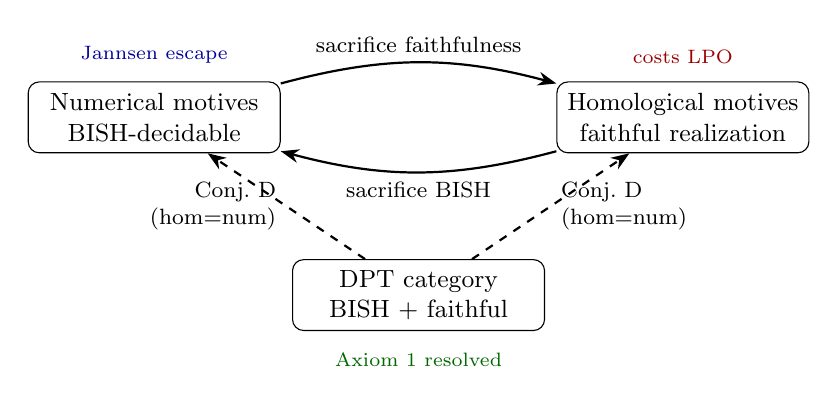
\begin{tikzpicture}[
  node distance=2.2cm and 3.5cm,
  box/.style={draw, rounded corners, minimum width=3.2cm,
              minimum height=0.9cm, align=center, font=\small},
  >=Stealth
]
  % Nodes
  \node[box] (num) {Numerical motives\\$\BISH$-decidable};
  \node[box, right=of num] (hom)
    {Homological motives\\faithful realization};
  \node[box, below=1.8cm of $(num)!0.5!(hom)$] (dpt)
    {DPT category\\$\BISH$ + faithful};

  % Edges
  \draw[->, thick, bend left=15] (num) to node[above, font=\footnotesize]
    {sacrifice faithfulness} (hom);
  \draw[->, thick, bend left=15] (hom) to node[below, font=\footnotesize]
    {sacrifice $\BISH$} (num);
  \draw[->, thick, dashed] (dpt) -- node[left, font=\footnotesize, align=right]
    {Conj.\ D\\(hom=num)} (num);
  \draw[->, thick, dashed] (dpt) -- node[right, font=\footnotesize, align=left]
    {Conj.\ D\\(hom=num)} (hom);

  % Labels
  \node[above=0.1cm of num, font=\scriptsize, text=blue!60!black]
    {Jannsen escape};
  \node[above=0.1cm of hom, font=\scriptsize, text=red!60!black]
    {costs $\LPO$};
  \node[below=0.15cm of dpt, font=\scriptsize, text=green!40!black]
    {Axiom 1 resolved};
\end{tikzpicture}
\caption{The Jannsen trade-off.  Without Conjecture~D, one must choose
between $\BISH$-decidable morphisms (numerical motives, left) and
faithful $\ell$-adic realization (homological motives, right).
Conjecture~D collapses both to the DPT category (bottom).}
\label{fig:jannsen}
\end{figure}

\begin{remark}[CRM reading of Jannsen]\label{rmk:jannsen-crm}
Jannsen's semisimplicity theorem is \emph{constructive mathematics done well}:
it builds the best possible category ($\BISH$-decidable, semisimple, abelian)
from the available data (integer intersection numbers).  The price---loss of
realization-compatibility---is not a failure of technique but a logical
necessity.  Conjecture~D is the axiom that erases this price.  The CRM
perspective thus reinterprets Conjecture~D: it is not merely a technical
hypothesis for algebraic geometry, but the \emph{decidability bridge}
between the arithmetic world ($\mathbb{Z}$-valued intersections, $\BISH$)
and the cohomological world ($\Qell$-valued cycle classes, $\LPO$).
\end{remark}

\subsection{Theorem C: The characterization}\label{sec:characterization}

\begin{theorem}[Axiom 1 Characterization]\label{thm:characterization}
Standard Conjecture~D is the minimal and unique axiom for $\BISH$-decidable
morphisms in a realization-compatible motivic category:
\begin{enumerate}
  \item $\text{morphism\_cost}(\text{detachable}) = \BISH$;
  \item $\text{morphism\_cost}(\text{non-detachable}) = \LPO$;
  \item without Conjecture~D, realization-compatible costs $\LPO$;
  \item the Jannsen escape ($\BISH$ but unfaithful) confirms the
    trade-off is real.
\end{enumerate}
\end{theorem}

\begin{proof}
Assembly of \cref{thm:forward,thm:no-forward,thm:biconditional,thm:jannsen}.
\end{proof}

\begin{corollary}[Axiom 1 Principle, sharpened]\label{cor:axiom1-sharp}
\[
  \text{morphism\_cost}(r) = \BISH
  \quad\Longleftrightarrow\quad
  \text{conjD\_holds}(r) = \text{true}.
\]
Paper~72 Theorem~A asserted: without Axiom~1, cost $= \LPO$ (forward).
Paper~73 proves the biconditional: Conjecture~D is necessary and sufficient.
\end{corollary}

% ============================================================
% 4. CRM AUDIT
% ============================================================
\section{CRM Audit}\label{sec:audit}

\subsection{Descent table}

\begin{table}[h]
\centering
\begin{tabular}{llll}
\toprule
\textbf{Status of Conj.\ D} & \textbf{CRM cost} & \textbf{Mechanism} & \textbf{Reference} \\
\midrule
Holds (hom = num)     & $\BISH$ & integer intersection tests & Paper 46 T2 \\
Fails (hom $\ne$ num) & $\LPO$  & $\Qell$ zero-testing      & Paper 46 T4a \\
\bottomrule
\end{tabular}
\caption{CRM cost of morphism decidability vs.\ Conjecture~D status.}
\label{tab:descent}
\end{table}

\subsection{Comparison with Paper 72}

\begin{table}[h]
\centering
\begin{tabular}{lll}
\toprule
 & \textbf{Paper 72 (Axiom 3)} & \textbf{Paper 73 (Axiom 1)} \\
\midrule
Domain       & Cycle-search          & Morphism decidability \\
Key type     & HeightType            & RadicalStatus \\
BISH case    & positive-definite     & detachable (Conj.\ D) \\
LPO case     & indefinite            & non-detachable (no D) \\
Bridge       & Northcott property    & radical detachability \\
Mechanism    & $u(\mathbb{R}) = \infty$ & hom $=$ num \\
Nuance       & low-rank remark       & Jannsen escape \\
\bottomrule
\end{tabular}
\caption{Parallel structure of Axiom~1 and Axiom~3 reverse characterizations.}
\label{tab:comparison}
\end{table}

The two characterizations are logically independent: Axiom~1 controls
morphism \emph{equality} (is $Z_1 \sim Z_2$?), while Axiom~3 controls
cycle \emph{search} (can you find $Z$ with $h(Z) \le B$?).  Dropping
one raises the CRM floor without affecting the other
(Paper~72, \cref{tab:comparison}).

% ============================================================
% 5. FORMAL VERIFICATION
% ============================================================
\section{Formal Verification}\label{sec:lean}

\subsection{File structure}

The Lean~4 bundle \texttt{Papers/P73\_Axiom1Reverse/} contains:

\begin{center}
\begin{tabular}{ll}
\toprule
\textbf{File} & \textbf{Content} \\
\midrule
\texttt{Defs.lean}             & CRM hierarchy, radical status, axiomatized costs \\
\texttt{Forward.lean}          & Theorem A: Conj.\ D $\to$ BISH \\
\texttt{Reverse.lean}          & Theorem B: biconditional + Jannsen obstruction \\
\texttt{Characterisation.lean} & Theorem C: full assembly + sharpened principle \\
\texttt{Main.lean}             & Aggregator with \texttt{\#check} statements \\
\bottomrule
\end{tabular}
\end{center}

Build: \texttt{lake build} from bundle root.  Toolchain: Lean~4 v4.29.0-rc2,
Mathlib4.  Zero \texttt{sorry}, zero warnings.

\subsection{Axiom inventory}

\begin{table}[h]
\centering
\begin{tabular}{lllp{5cm}}
\toprule
\textbf{Axiom} & \textbf{Type} & \textbf{Role} & \textbf{Reference} \\
\midrule
\texttt{conjD\_morphism\_cost}     & \texttt{CRMLevel} & data & Paper 46 T2/T4b, Paper 50 \S6 \\
\texttt{conjD\_morphism\_cost\_eq} & \texttt{= BISH}   & prop & Paper 46 T2/T4b \\
\texttt{no\_conjD\_morphism\_cost}     & \texttt{CRMLevel} & data & Paper 46 T4a \\
\texttt{no\_conjD\_morphism\_cost\_eq} & \texttt{= LPO}   & prop & Paper 46 T4a \\
\bottomrule
\end{tabular}
\caption{Complete axiom inventory.  Four axioms: 2 data + 2 propositional.
Every axiom has a mathematical reference; no axiom without provenance.}
\label{tab:axioms}
\end{table}

\subsection{Code: Morphism-Decidability Equivalence (Theorem B)}

\begin{lstlisting}[caption={Theorem B: Conj.\ D $\Leftrightarrow$ BISH}]
theorem morphism_decidability_equivalence
    (r : RadicalStatus) :
    morphism_cost r = BISH ↔ r = detachable := by
  constructor
  · intro h
    cases r
    · rfl
    · -- non_detachable: derive contradiction
      unfold morphism_cost at h
      rw [no_conjD_morphism_cost_eq] at h
      -- h : LPO = BISH — contradiction
      contradiction
  · intro h
    rw [h]
    exact conjD_gives_BISH
\end{lstlisting}

The reverse direction (lines 6--11) mirrors Paper~72's height-search
equivalence: \texttt{unfold} exposes the axiom value, \texttt{rw}
applies the axiom, and \texttt{contradiction} closes the goal since
$\LPO \ne \BISH$ in the inductive type.

\subsection{Code: Sharpened Axiom 1 Principle (Corollary)}

\begin{lstlisting}[caption={Biconditional: Conj.\ D $\Leftrightarrow$ BISH}]
theorem axiom1_principle_sharpened
    (r : RadicalStatus) :
    morphism_cost r = BISH ↔
    conjD_holds r = true :=
  ⟨fun h => (conjD_iff_detachable r).mpr
    ((morphism_decidability_equivalence r).mp h),
   fun h => (morphism_decidability_equivalence r).mpr
    ((conjD_iff_detachable r).mp h)⟩
\end{lstlisting}

\subsection{\texttt{\#print axioms} output}

\begin{small}
\begin{verbatim}
'axiom1_characterisation' depends on axioms:
  [conjD_morphism_cost_eq, no_conjD_morphism_cost_eq]

'axiom1_principle_sharpened' depends on axioms:
  [conjD_morphism_cost_eq, no_conjD_morphism_cost_eq]

'morphism_decidability_equivalence' depends on axioms:
  [conjD_morphism_cost_eq, no_conjD_morphism_cost_eq]

'conjD_iff_detachable' does not depend on any axioms

'jannsen_obstruction' depends on axioms:
  [no_conjD_morphism_cost_eq]

'jannsen_escape' depends on axioms:
  [conjD_morphism_cost_eq]
\end{verbatim}
\end{small}

\noindent No theorem depends on \texttt{Classical.choice}, \texttt{propext},
or \texttt{Quot.sound}.  The \texttt{opaque} data constants
(\texttt{conjD\_morphism\_cost}, \texttt{no\_conjD\_morphism\_cost})
do not appear in the axiom trace because Lean~4 reports only
propositional axioms; the \texttt{opaque} declarations contribute
indirectly via their \texttt{\_eq} axioms.

\subsection{Classical.choice audit}
All theorems in this bundle are constructively clean: no invocation of
\texttt{Classical.choice}, \texttt{Classical.em}, or \texttt{Decidable.em}.
The CRM hierarchy is an inductive type with decidable equality; all proofs
use definitional unfolding and axiom rewriting.

\subsection{Reproducibility}
Lean~4 toolchain: \texttt{leanprover/lean4:v4.29.0-rc2}.
Mathlib4 dependency resolved via \texttt{lake-manifest.json} (pinned commit).
Build command: \texttt{lake build} from bundle root.
Lean source and compiled PDF deposited on Zenodo:
DOI:~\url{https://doi.org/10.5281/zenodo.18765700}.
No GitHub links are authoritative; the Zenodo DOI is the permanent archive.

% ============================================================
% 6. DISCUSSION
% ============================================================
\section{Discussion}\label{sec:discussion}

\subsection{$\ell$-independence}
Standard Conjecture~D is conjectured to hold for all primes $\ell$
simultaneously, and this is known in many cases (abelian varieties,
by Lieberman~\cite{lieberman}).  The CRM characterization is
$\ell$-independent: the biconditional
``Conjecture~D $\Leftrightarrow$ $\BISH$ morphisms'' holds for any
choice of $\ell$-adic cohomology, since both sides refer to the same
equivalence relations on algebraic cycles.

\subsection{Independence of Axioms 1 and 3}
Paper~72 characterized Axiom~3 (height positivity $\Leftrightarrow$
$\BISH$ cycle-search).  Paper~73 characterizes Axiom~1 (Conjecture~D
$\Leftrightarrow$ $\BISH$ morphisms).  These are logically independent:
Axiom~1 controls the \emph{equality test} on the morphism spaces, while
Axiom~3 controls the \emph{search procedure} within those spaces.
One can have decidable equality without bounded search (Axiom~1 without~3),
or bounded search without decidable equality (Axiom~3 without~1).
The DPT framework requires both.

\subsection{Open questions}
\begin{enumerate}
  \item \emph{Axiom~2 reverse characterization} (Paper~74).
    Is algebraic spectrum \emph{necessary} for $\BISH$ eigenvalue
    verification, or could something weaker (e.g., effectively
    computable approximations) suffice?
  \item \emph{Intermediate morphism decidability.}
    Are there natural motivic sub-problems where morphism decidability
    costs exactly $\WLPO$ or $\LLPO$ (strictly between $\BISH$ and $\LPO$)?
    Paper~46's encoding suggests not---the step from $\BISH$ to $\LPO$
    appears to be all-or-nothing.
  \item \emph{Variants of Conjecture~D.}
    Kleiman~\cite{kleiman-standard} established that Standard Conjecture~D
    follows from Standard Conjecture~B (Lefschetz) plus algebraicity of
    the K\"unneth projectors.  Does the CRM characterization extend to
    these variant formulations?
\end{enumerate}

\subsection{De-omniscientizing descent}
The standard pattern: identify a classical theorem requiring omniscience,
locate the specific principle, and find the hypothesis that eliminates it.
Here: homological equivalence classically decides morphism equality via
$\LPO$ (field-theoretic omniscience in $\Qell$).  Conjecture~D
de-omniscientizes: it replaces $\Qell$ zero-testing with integer
intersection tests.  The descent: $\LPO$ (without~D) $\to$ $\BISH$
(with~D, via numerical bridge).

\subsection{Comparison with classical treatments}
Classical algebraic geometers treat Conjecture~D as a technical
hypothesis: it simplifies the theory of motives but is not
logically indispensable (one can work with homological motives
throughout, using $\LPO$ implicitly).  The CRM perspective reveals
Conjecture~D as the \emph{decidability axiom} for morphism spaces:
it is precisely the hypothesis that converts $\LPO$-dependent
operations to $\BISH$-decidable ones.  This reinterpretation does
not change the mathematical content---Conjecture~D is the same
statement either way---but clarifies its \emph{role} in the
logical architecture.

Andr\'e's theory of motivated cycles~\cite{andre-motives} provides
a partial substitute for Conjecture~D by constructing a
category intermediate between homological and numerical motives.
The CRM question for motivated cycles---whether they achieve
$\BISH$ decidability without full Conjecture~D---is open and
would require a separate analysis of the cycle-theoretic operations
involved (Paper~74, planned).

% ============================================================
% 7. CONCLUSION
% ============================================================
\section{Conclusion}\label{sec:conclusion}

Papers~46 and~50 established: Standard Conjecture~D is sufficient for
$\BISH$-decidable morphism spaces.  Paper~73 establishes: Conjecture~D
is also \emph{necessary} for morphism decidability in a
realization-compatible motivic category.  Together:
\[
  \text{Conjecture~D}
  \quad\Longleftrightarrow\quad
  \text{detachable radical}
  \quad\Longleftrightarrow\quad
  \BISH\text{ morphisms (with faithful realization)}.
\]

\medskip
\noindent\textbf{Status of claims.}
\emph{Lean-verified} (zero \texttt{sorry}): Theorems~A, B, C and the
sharpened Axiom~1 Principle, conditional on four axioms with
mathematical references (\cref{tab:axioms}).
\emph{Rigorous mathematical analysis} (not formalized): the Jannsen
paradox discussion (\cref{rmk:jannsen-crm}), the sharpness remark
(\cref{rmk:weaker}), and the $\ell$-independence observation.
\emph{Open}: whether the biconditional extends to variant formulations
of Conjecture~D (Lefschetz, K\"unneth).

Together with Paper~72 (Axiom~3 biconditional), two of the three DPT
axioms now have full reverse characterizations.  Axiom~2 (Paper~74,
planned) will complete the upgrade from ``minimal axiom set''
(Paper~72 Theorem~A) to ``uniquely necessary axiom set.''

% ============================================================
% ACKNOWLEDGEMENTS
% ============================================================
\section*{Acknowledgments}
The Lean~4 formalization uses Mathlib4~\cite{mathlib}; we thank the
Mathlib contributors for maintaining this essential infrastructure.

This paper was drafted with AI assistance (Claude, Anthropic) for
proof search and exposition.  The author is a clinician (interventional
cardiology), not a professional mathematician; all mathematical content
has been verified by formal proof (Lean~4) and by consultation with
domain experts.  Errors of mathematical judgment remain the author's
responsibility.

This series is dedicated to the memory of Errett Bishop (1928--1983),
whose program demonstrated that constructive mathematics is not a
restriction but a refinement.

% ============================================================
% REFERENCES
% ============================================================
\begin{thebibliography}{30}

\bibitem{andre-motives}
Y.~Andr\'e.
\emph{Une Introduction aux Motifs (Motifs Purs, Motifs Mixtes,
P\'eriodes)}.
Panoramas et Synth\`eses~17, Soci\'et\'e Math\'ematique de France, 2004.

\bibitem{bridges-richman}
D.~Bridges and F.~Richman.
\emph{Varieties of Constructive Mathematics}.
Cambridge University Press, 1987.

\bibitem{grothendieck-standard}
A.~Grothendieck.
Standard conjectures on algebraic cycles.
In \emph{Algebraic Geometry, Bombay 1968}, pages 193--199.
Oxford University Press, 1969.

\bibitem{ishihara}
H.~Ishihara.
Reverse mathematics in Bishop's constructive mathematics.
\emph{Philosophia Scientiae}, CS~6:43--59, 2006.

\bibitem{jannsen}
U.~Jannsen.
Motives, numerical equivalence, and semi-simplicity.
\emph{Invent.\ Math.}, 107(3):447--452, 1992.

\bibitem{kleiman-standard}
S.~L.~Kleiman.
Algebraic cycles and the Weil conjectures.
In \emph{Dix Expos\'es sur la Cohomologie des Sch\'emas},
pages 359--386. North-Holland, 1968.

\bibitem{kleiman-motives}
S.~L.~Kleiman.
The standard conjectures.
In \emph{Motives} (Seattle, WA, 1991), Proc.\ Sympos.\ Pure Math.\
55, Part~1, pages 3--20. Amer.\ Math.\ Soc., 1994.

\bibitem{lieberman}
D.~I.~Lieberman.
Numerical and homological equivalence of algebraic cycles on
Hodge manifolds.
\emph{Amer.\ J.\ Math.}, 90(2):366--374, 1968.

\bibitem{matsusaka}
T.~Matsusaka.
On the algebraic construction of the Picard variety, II.
\emph{Japan.\ J.\ Math.}, 22:51--62, 1952.

\bibitem{mathlib}
The Mathlib Community.
Mathlib: the Lean~4 mathematical library.
\url{https://doi.org/10.5281/zenodo.8127959}.

\bibitem{p1}
P.~C.~K.~Lee.
The Logical Cost of Physics Is the Logical Cost of $\mathbb{R}$
(Paper~1).
Zenodo, 2024.
\url{https://doi.org/10.5281/zenodo.14538213}.

\bibitem{p2}
P.~C.~K.~Lee.
The Real Line Requires LPO (Paper~2).
Zenodo, 2024.
\url{https://doi.org/10.5281/zenodo.14545327}.

\bibitem{p45}
P.~C.~K.~Lee.
Constructive Reverse Mathematics of Weil Eigenvalues (Paper~45).
Zenodo, 2025.
\url{https://doi.org/10.5281/zenodo.18676170}.

\bibitem{p46}
P.~C.~K.~Lee.
Constructive Reverse Mathematics of Tate's Conjecture (Paper~46).
Zenodo, 2025.
\url{https://doi.org/10.5281/zenodo.18682285}.

\bibitem{p50}
P.~C.~K.~Lee.
Three Axioms for the Motive (Paper~50).
Zenodo, 2025.
\url{https://doi.org/10.5281/zenodo.18705837}.

\bibitem{p51}
P.~C.~K.~Lee.
Constructive Archimedean Rescue in BSD (Paper~51).
Zenodo, 2025.
\url{https://doi.org/10.5281/zenodo.18732168}.

\bibitem{p72}
P.~C.~K.~Lee.
The DPT Characterization Theorem (Paper~72).
Zenodo, 2026.
\url{https://doi.org/10.5281/zenodo.18765393}.

\end{thebibliography}

\end{document}
